%% LaTeX2e class for student theses
%% thesis.tex
%% 
%% Karlsruhe Institute of Technology
%% Institute for Program Structures and Data Organization (IPD)
%% Chair for Software Design and Quality (SDQ)
%%
%% Dr.-Ing. Erik Burger
%% burger@kit.edu
%%
%% Version 1.1, 2014-11-21

%% Available languages: english,ngerman
%% Available modes: draft,final (see README)
\documentclass[english]{sdqthesis}
%% ---------------------------------
%% | Information about the thesis  |
%% ---------------------------------

%% Name of the author
\author{Daniel H. Draper}

%% Title (and possibly subtitle) of the thesis
\title{Online Neural Network-based Language Identification}

%% Type of the thesis 
\thesistype{Master's Thesis}

%% Change the institute here, ``IPD'' is default
\myinstitute{Institute for Anthropomatics and Robotics}

%% You can put a logo in the ``logos'' directory and include it here
%% instead of the SDQ logo
% \grouplogo{myfile}
%% Alternatively, you can disable the group logo
\nogrouplogo

%% The reviewers are the professors that grade your thesis
\reviewerone{Prof. Dr. Alexander Waibel}
%\reviewertwo{Prof. B}

%% The advisors are PhDs or Postdocs
\advisorone{M.Sc. Markus Müller}
%% The second advisor can be omitted
\advisortwo{Dr. Sebastian Stüker}

%% Please enter the start end end time of your thesis
\editingtime{12. December 2016}{11. May 2017}

\settitle

%% --------------------------------
%% | Settings for word separation |
%% --------------------------------

%% Describe separation hints here.
%% For more details, see 
%% http://en.wikibooks.org/wiki/LaTeX/Text_Formatting#Hyphenation
\hyphenation{im-ple-men-ta-tion
% me-ta-mo-del
}

%% --------------------------------
%% | Bibliography                 |
%% --------------------------------

%% Use biber instead of BibTeX, see README
%\usepackage[citestyle=numeric,style=numeric,backend=biber]{biblatex}
\usepackage{xr}
\usepackage{listings}
\usepackage{pdfpages}
\usepackage[nopostdot,nonumberlist,toc]{glossaries}
\usepackage{tikz}
\usepackage{pgfplots}
\usepackage{arydshln}
\pgfplotsset{width=10cm,compat=1.9} 
\newcommand{\ltab}{\raggedright\arraybackslash}
\setlength{\parskip}{.5em}
\DeclareMathOperator*{\argmax}{arg\,max}
\lstdefinelanguage{tclfix}% from tcl definition
   {alsoletter={.:,*=&-},%
     morekeywords={after,append,array,names,exists,anymore,donesearch,%
       get,nextelement,set,size,startsearch,auto_mkindex,binary,break,%
       case,catch,cd,clock,close,concat,console,continue,default,else,%
       elseif,eof,error,eval,exec,-keepnewline,exit,expr,fblocked,%
       fconfigure,fcopy,file,atime,dirname,executable,exists,extension,%
       isdirectory,isfile,join,lstat,mtime,owned,readable,readlink,%
       rootname,size,stat,tail,type,writable,-permissions,-group,-owner,%
       -archive,-hidden,-readonly,-system,-creator,-type,-force,%
       fileevent,flush,for,foreach,format,gets,glob,global,history,if,%
       incr,info,argsbody,cmdcount,commands,complete,default,exists,%
       globals,level,library,locals,patchlevel,procs,script,tclversion,%
       vars,interp,join,lappend,lindex,linsert,list,llength,lrange,%
       lreplace,lsearch,-exact,-regexp,-glob,lsort,-ascii,-integer,%
       -real,-dictionary,-increasing,-decreasing,-index,-command,load,%
       namespace,open,package,forget,ifneeded,provide,require,unknown,%
       vcompare,versions,vsatisfies,pid,proc,puts,-nonewline,pwd,read,%
       regexp,-indices,regsub,-all,-nocaserename,return,scan,seek,set,%
       socket,source,split,string,compare,first,index,last,length,match,%
       range,tolower,toupper,trim,trimleft,trimright,subst,switch,tell,%
       time,trace,variable,vdelete,vinfo,unknown,unset,uplevel,upvar,%
       vwait,while,acos,asin,atan,atan2,ceil,cos,cosh,exp,floor,fmod,%
       hypot,log,log10,pow,sin,sinh,sqrt,tan,tanh,abs,double,int,round%
     },%
     morestring=[d]",%
%   MoreSelectCharTable=%   <= the strange definition
%   \lst@CArgX\#\relax\lst@DefDelimB{}{}%
%   {\ifx\lst@lastother\lstum@backslash
%     \expandafter\@gobblethree
%     \fi}%
%   \lst@BeginComment\lst@commentmode
%   {{\lst@commentstyle}\lst@Lmodetrue}%
     morecomment=[l]\#     % <= this one ! Much simpler
   }[keywords,comments,strings]%

\lstset{commentstyle=\itshape,language=tclfix}

\makeglossaries
%% ====================================
%% ====================================
%% ||                                ||
%% || Beginning of the main document ||
%% ||                                ||
%% ====================================
%% ====================================
\begin{document}
%% Set PDF metadata
\setpdf

%% Set the title
\maketitle

%% The Preamble begins here
\frontmatter

%% LaTeX2e class for student theses: Declaration of independent work
%% sections/declaration.tex
%% 
%% Karlsruhe Institute of Technology
%% Institute for Program Structures and Data Organization
%% Chair for Software Design and Quality (SDQ)
%%
%% Dr.-Ing. Erik Burger
%% burger@kit.edu
%%
%% Version 1.1, 2014-11-21

\thispagestyle{empty}
\null\vfill
\noindent\hbox to \textwidth{\hrulefill} 
\iflanguage{english}{I declare that I have developed and written the enclosed
thesis completely by myself, and have not used sources or means without
declaration in the text.}%
{Ich versichere wahrheitsgemäß, die Arbeit
selbstständig angefertigt, alle benutzten Hilfsmittel vollständig und genau
angegeben und alles kenntlich gemacht zu haben, was aus Arbeiten anderer
unverändert oder mit Änderungen entnommen wurde.}
 
 
%% ---------------------------------------------
%% | Replace PLACE and DATE with actual values |
%% ---------------------------------------------
\textbf{Karlsruhe, 11th of May, 2017}
\vspace{1.5cm}
 
\dotfill\hspace*{8.0cm}\\
\hspace*{2cm}(\theauthor) 
\cleardoublepage

\setcounter{page}{1}
\pagenumbering{roman}

%% ----------------
%% |   Abstract   |
%% ----------------

%% For theses written in English, an abstract both in English
%% and German is mandatory.
%%
%% For theses written in German, a German abstract is sufficient.
%%
%% The text is included from the following files:
%% - sections/abstract

\includeabstract

%% ------------------------
%% |   Table of Contents  |
%% ------------------------
\tableofcontents

\listoffigures
\listoftables

%% -----------------
%% |   Main part   |
%% -----------------

\mainmatter

%% LaTeX2e class for student theses
%% sections/content.tex
%% 
%% Karlsruhe Institute of Technology
%% Institute for Program Structures and Data Organization
%% Chair for Software Design and Quality (SDQ)
%%
%% Dr.-Ing. Erik Burger
%% burger@kit.edu
%%
%% Version 1.1, 2014-11-21

\chapter{Introduction}
\label{ch:Introduction}
Language Identification (LID) describes the classification task of differentiating between spoken speech in different languages and being able to correctly classify which speech-segments consists of which language.  Neural Networks refer to Artificial Neural Network's, a Machine Learning approach to classification tasks. They are employed greatly throughout all sciences and especially in computer science and tasks concerned with the processing of spoken speech. This thesis tries to find a low-latency, fast, or ``online'', approach to Language Identification using the classification method of neural networks.

The work done in this thesis uses the Janus Recognition Toolkit (jrtk)\footnote{Janus Recognition Toolkit:~\url{http://isl.anthropomatik.kit.edu/cmu-kit/english/1406.php}}, an Automatic Speech Recognition toolkit developed in joint cooperation by the KIT and CMU. The jrtk offers a tcl/tk\footnote{Tcl/tk:~\url{https://www.tcl.tk/}} script-based environment for the development of Automatic Speech Recognition systems, therefore source code in this thesis will consist of tcl/tk scripts with (some) janus-specific commands. The jrtk and tcl/tk are further explained in sec.~\ref{sec:fund:jrtk}.

\section{Motivation}
\label{sec:Introduction:Motivation}
Automatic Speech Recognition (ASR) is used in many applications and devices today, especially in the rise of handheld mobile devices like smartphones and tablets. It has progressed quickly in the last five years and has found commercial success. Famous examples include Google\footnote{Google: \url{www.google.com}}'s ``Ok, Google'' and Apple\footnote{Apple: \url{www.apple.com}}'s Siri. Which both include voice search\cite{franz2008voice} and a form of voice control, that even is extensible in the case of Google and Android e.g\cite{voicecontrol2014}. Many other applications have emerged, including spoken language translation\footnote{IWSLT: \url{iwslt.org}}, especially relevant for this thesis in the realm of Lecture Translation\cite{lecturetranslator2016} .

The task of Language Identification can be applied in all of those fields, as Automatic Speech Recognition is mostly trained on one language and therefore requires a totally different setup of classifiers per language, making a manual change of language previous to recognition necessary. Robust and low-latency language identification would eliminate the need for this.

LID would be especially applicable in the realm of spoken language translation, as used for example in the European Parliament where already components of ASR and Machine Translation are employed and are being actively developed in the TC-STAR inititative\footnote{TC-STAR: \url{tcstar.org}}, e.g as in\cite{vilar2005statistical}, and LID would further be able to automate these translation tasks.

This thesis will focus mostly on the KIT's lecture Translator\footnote{Lecture Translator: \url{https://lecture-translator.kit.edu}}  as the system trained was implemented for it. We believe our results are generic enough to be transferable to other applications with small implementation-specific changes.

\section{Overview}
\label{sec:Intro:Overview}

The rest of this thesis is set up as follows: Chapter 2 introduces related and previous work in the realm of Language Identification. The following chapter 3 gives an introductory view of Language Identification, and introduces the task this thesis tries to solve. Afterwards we give preliminary theoretical explanations and definitions, including an introduction to Neural Networks in Sec.~\ref{sec:fund:NN}. Chapter 4 describes the experimental setup used in this thesis, including the data corpora. Audio Preprocessing is explained in detail in Chapter 5.

Chapters 6 desribes our results that were accomplished by experimenting on network setup and layout. Different smoothing mechanisms on top of the direct neuronal output layer of the network are explained in chapter 7. This is followed by the final summary of our work and a future work outlook in chapter 8.
%% LaTeX2e class for student theses
%% sections/preliminary.tex
%% 
%% Karlsruhe Institute of Technology
%% Institute for Program Structures and Data Organization
%% Chair for Software Design and Quality (SDQ)
%%
%% Dr.-Ing. Erik Burger
%% burger@kit.edu
%%
%% Version 1.1, 2014-11-21

\chapter{Related Work}
\label{ch:Related Work}
This chapter introduces related and previous works in the realm of language identification and how their approaches differ from the ones employed in the following chapters.

\chapter{Fundamentals}
\label{ch:fund}

The following chapter will define and explain terms and concepts used throughout this thesis, as to make understanding of the following chapters easier.

\section{Janus Recognition Toolkit (jrtk)}
\label{sec:fund:jrtk}
The Janus Recognition Toolkit (jrtk) also known as just ``Janus'' is a general-purpose speech recognition toolkit developed in joint cooperation by both the Carnegie Mellon University Interactive Systems Lab and the Karlsruhe Institute of Technology Interactive Systems Lab~\cite{lavie1997janus}. Part of janus and the jrtk are a speech-to-speech translation system which includes Janus-SR the speech recognition component, the main part of janus used in this thesis. 

Developed to be flexible and extensible, the jrtk can be seen as a programmable shell with janus functionality being accessible through objects in the tcl/tk scripting language. It features the IBIS decoder, that uses Hidden Markov Models for acoustic modeling in general, although in this thesis we used a neural network as our speech recognizer to generate the input features required by our Language ID network.

This thesis makes extensive use of the jrtk's and tcl/tk's scripting capabilities to be able to pre-process speech audio files for further use by our experimental setup. It also uses tcl/tk scripts and it's janus API functionality in the development of our smoothing and evaluation scripts as can be seen in Ch.~\ref{ch:eval}.
\section{Neural Networks}
\label{sec:fund:NN}
Artificial Neural Networks today are used in many different fields: from image recognition/face recognition in~\cite{lawrence1997face} to Natural Language Processing in~\cite{collobert2008unified} and, as relevant to this thesis, to Speech Recognition and very successfully as in~\cite{hinton2012deep}. It has also been used in the realm of Language Identification, which will be described in Sec.~\ref{sec:fund:work}. This section will provide fundamental knowledge of how neural networks work and how to train them, to make the understanding of later chapters easier for the reader. The information in this section is based mostly on~\cite{haykin2004comprehensive}, ~\cite{Goodfellow-et-al-2016} and~\cite{deeplearning-online}


\subsection{General Setup}
\label{sec:fund:general}
Neural Networks are based on collections of small ''neural units``  working together in tandem. The neuron's behavior can be loosely linked to the brain's axons. Each neuron is connected with others and a neuron is ''stimulated`` by input on these connections and then decides on its own activation, or stimulation, by using a summation, or threshold, function with a certain limit to decide if the neuron ''fires`` and its own activation is propagated through the network to adjacent units. By changing weigths and activation thresholds in the network its output changes, therefore the possible adjustable parameter set \(\Theta\) for a neural network includes all the weights for all neurons as well as all thresholds for the activation functions in each neuron.

\subsection{Artificial Neuron}
\label{sec:fund:AN}

An artificial neuron, or perceptron in its most basic form, is a mathematical function that consists of four parameters that can be adjusted independently from each other:
\begin{itemize}
\item \(w_i\) the input weights for all inputs
\item \(\Sigma\) the transfer function for summation of the weighted inputs
\item \(\varphi\) the activation function that calculates the output value \(y_k\) basend on the transfer input and the threshold
\item \(\theta\) the threshold which defines when the neuron activates.
\end{itemize}

This means an artificial neuron with output \(y_k\) is the function~\ref{eq:an}. Many of these neurons coupled together (via the output of a neuron on a previous layer becoming the input for one on the current layer), make an Artificial Neural Network as used in this thesis. A schematic drawing of this can be seen in Fig.~\ref{fig:neuron}.

\begin{equation}
y_k = \varphi(\sum_{j=0}^{m} w_{kj}x_j) - \theta_j
\label{eq:an}
\end{equation}

\begin{figure}[h!]
\label{fig:neuron}
\caption{A schematic drawing of a Neuron and it's parameters}
\centering
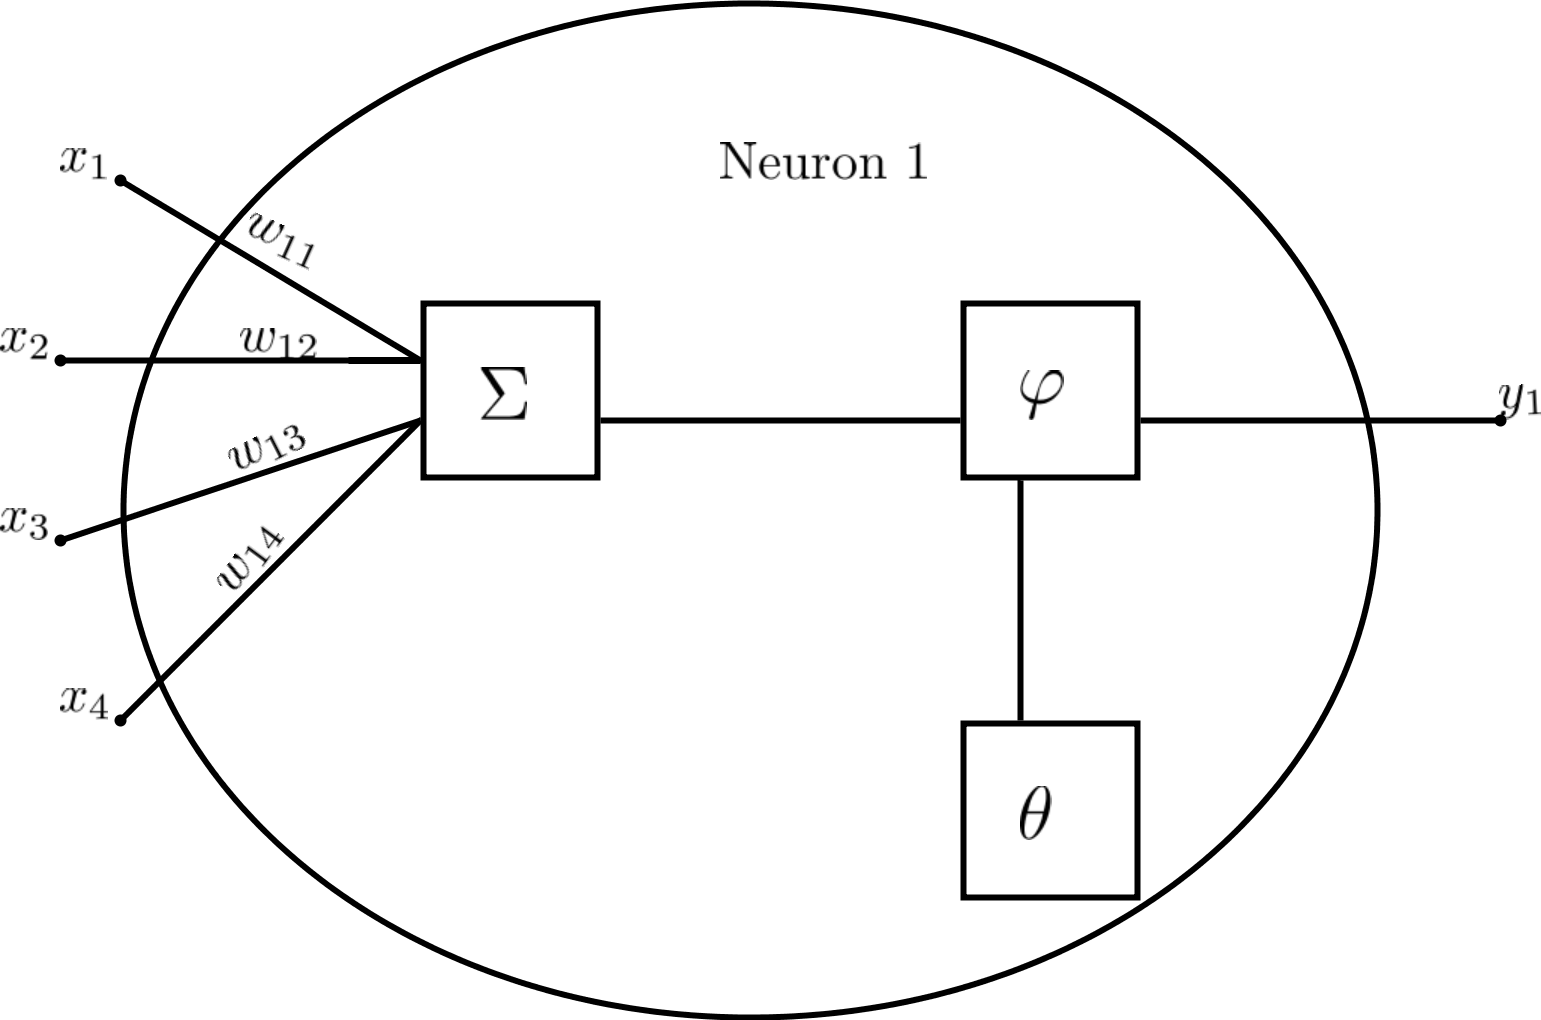
\includegraphics[width=0.7\textwidth]{images/neuron.png}
\end{figure}

\subsection{General Network Setup}
\label{sec:fund:netSetup}

A basic neural network consists of three layers: the input, a hidden layer of neurons and the output layer. Hereby, the output layer consists of as many neurons as classes that the network is trying to classify against and the one with the highest activation after entering input, is the classification output of the net.  A basic, fully-connected (referring to the connections between neurons, so fully-connected means each neuron is connected to each possible other neuron) net can be seen in Fig.~\ref{fig:net}.

\begin{figure}
\label{fig:net}
\caption{A schematic drawing of a neural network}
\centering
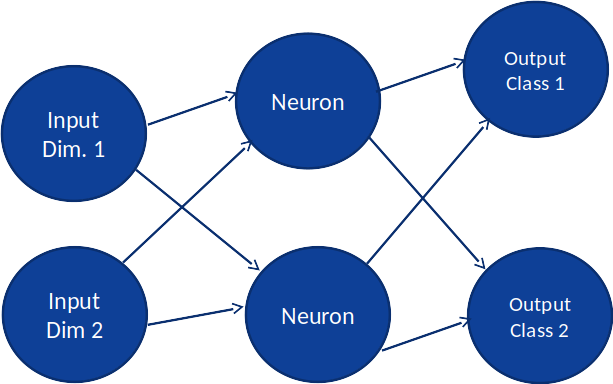
\includegraphics{images/net.png}
\end{figure}

\subsection{Network Types}
\label{sec:fund:types}

\subsubsection{Feed-Forward Neural Networks}
A basic (non-deep) \textit{Feed-Forward Neural Network} consists of three layers: the input, a hidden layer of neurons and the output layer. Feed-Forward refers to the fact, in opposition to \textit{Recurrent Neural Networks}, that connections between the neural units are not cyclic. 

In such a basic network, the output layer consists of as many neurons as classes that the network is trying to classify against and the neuron with the highest activation after entering input, is the classification output of the net.

\subsubsection{Deep Feed-Forward Neural Networks}
\textit{Deep Feed-Forward Neural Networks}, DNNs, the net-type most used in this thesis, refer to Networks that have more than one hidden layer between input and output, but still feature non-cyclic connections between neurons. DNNs have a better performance than single-hidden-layer-networks in general, but require different techniques for training. 

A common description of this phenomen is, that each hidden layer increases the level of abstraction the network can manage. E.g, in image processing, if the first layer recognizes a color in a certain pixel, then the next layer can infer more abstract characteristics from the output of the first layer. For example, after knowing a certain pixel is dark the next layer can derive that area might be the eye in a picture of a face, etc. This obviously makes more complicated classification tasks possible but also makes learning algorithms more difficult.

\subsubsection{Deep Recurrent Neural Networks}
\textit{Deep Recurrent Neural Networks}, RNNs, refer to neural networks that are DNN's but cyclic connections are allowed. This means the network can have temporal behavior, so its performance changes dynamically over time, when the state of later neurons changes and affects the neurons in previous layers.


\subsection{Learning}
\label{sec:fund:Learn}
The interesting part about Neural Networks is their ability to learn from data and improve their own performance. Improving performance in this case means that by adjusting the available parameters of the neurons part of the network, we minimize a cost function that describes the difference between an optimal output and the actual output. 

A Network can be seen to be an approximation of a function \(f^*\). So, a network trying to classify an input \(x\) into a class \(y\) approximates:
\begin{equation}
\label{eq:learn}
y=f^*(x)
\end{equation}
Then one run of the Network with parameter set \(\Theta\) gives the mapping \(y = f(x;\Theta)\) and we are trying to minimize our cost function of \(C= f^* - f\) by adjusting the set of parameters in \(\Theta\) each run.

\paragraph{Three basic approaches exist for training a network:} \hspace{0pt} \\
\begin{itemize}
\item \textit{Supervised Training}, where the optimal output for input train data is known. This means, the train data has been pre-classified by a ``teacher''. This is the method we use in this thesis and further explained below.
\item \textit{Reinforcement Training}, where the optimal input for train data is not known prior to training, but the environment gives the net feedback about its own output and good output is ``reinforced'' while bad output is discouraged.
\item \textit{Unsupervised Training}, where nothing is known about the environment and the net (often) just tries to learn the probabilistic distribution of the data.
\end{itemize}

\subsubsection{Sampling}
\label{sec:fund:Sampling}

Data for training is generally split into three sets: the training set with a size of about \(80\%\) of the total available data which is then used for the training, the development set with a size of about \(10\%\) used for evaluation of the net and adjusting different parameters without ``distorting'' the last test set which also has a size of around \(10\%\) and is used for final ``clean'' validation of the net performance.

Sampling is most commonly, as in this thesis, done using the 

\subsubsection{Supervised Training}
\label{sec:fund:ST}
Supervised Training refers to training where the optimal output for the training data is known, so a classification of the train data exists prior to training. This makes calculation of the Cost function as defined in the previous section relatively easy, as we define \(C\) as the actual difference in output of the current net with current parameter set \(\Theta\) compared to the teacher-defined classification/labeling. 

\paragraph{Mean Squared Error Function}

One way to calculate the difference between the net and the teacher-classification is by using the mean squared error, as is used in the training of nets in this thesis. If  \(t\) is the expected output and \(f(x;\Theta)\) is the actual predicted output and \(M\) the number of output neurons/classes, we define the Mean Squared Error (MSE) as:
\begin{equation}
E = 1 / 2 \sum_{j=1}^{M}(f(x;\Theta) - t)^2
\end{equation}

\paragraph{Stochastic Gradient Descent} The goal of course is to minimize the MSE as defined above by adjusting parameters for each neuron and layer (including weights to output neurons) to change the predicted output of the net.  This is done by adjusting the weights in direction of the falling gradient for each weight.
\begin{equation}
w_{i+1} = w_i - \eta \nabla E(f(x;w), t) = w_i - \eta \nabla 1/2\sum_{j=1}^M(f(x;w) - t)^2
\end {equation}

This method is called the ``Gradient Descent'', with \(\eta\) being the ``Learning Rate'', the freely adjustable speed at which the network changes and therefore learns. As calculation of this gradient for every sample in the training data set is expensive, a stochastic approach is used where only a small number of samples is used each iteration to calculate the gradient, as the relation between the change of the mean error and the value of samples is not linear. Therefore the calculation of the ´´Stochastic Gradient Descent'' (SGD) is enough to estimate the real required parameter-changes.

\paragraph{Backpropagation} While the SGD is used to calculate each iterative weight according to the falling gradient, the Backpropagation algorithm is used to calculate each weight from the total output of the net and its input. If we have neural network output vector (all output neurons together) \(t_i\), input vector (all input dimensions together) \(x_i\) and current weights \(w_i\) we can calculate \(w_{i+1}\) by calculating the SGD on the function \(w \rightarrow E(w, x_i), y_i)\).

With preceding definitions we can summarize the training algorithm of a DNN as follows:
\definecolor{green}{rgb}{0.0, 0.4, 0.13}
\lstset{captionpos=b,tabsize=3,frame=lines,keywordstyle=\color{blue},commentstyle=\color{green},stringstyle=\color{red},numbers=left,numberstyle=\tiny,numbersep=5pt,breaklines=true,showstringspaces=false,basicstyle=\footnotesize,emph={label}}
\begin{lstlisting}[label=lst:pseudo:train,caption=Pseudo Code to show the Backpropagation/SGD algorithm in Action,mathescape]
 $\displaystyle w_0 := rand()$
  do
     forEach train-sample s
        $\displaystyle f(x;w_i)$ = neural-net-output$\displaystyle(w_i, s) $ // Actual calculation using each neurons output -> Forward pass
        t = pre-classification(s)
        Error = $\displaystyle E(f(x;w_i), t)$
         $ \displaystyle w_{i+1}:=  w_i - \eta \nabla E(f(x;w), t) = w_i - \eta \nabla 1/2\sum_{j=1}^M(f(x;w) - t)^2$  //For all Weights and layers -> Backwards pass
        $\displaystyle w :=w_{i+1}$
   if ($\Delta E$ <= Threshold) break
return Net
\end{lstlisting}

%% LaTeX2e class for student theses
%% sections/content.tex
%% 
%% Karlsruhe Institute of Technology
%% Institute for Program Structures and Data Organization
%% Chair for Software Design and Quality (SDQ)
%%
%% Dr.-Ing. Erik Burger
%% burger@kit.edu
%%
%% Version 1.1, 2014-11-21

%To be able to reference labels in other file
\externaldocument{introduction}
\externaldocument{appendix}


\chapter{Experimental Setup}
\label{ch:LITasks}

This chapter lays out the experimental setup used in this thesis. While Language Identification is applicable in many different scenarios, here the focus lies on trying to establish a low-latency online approach for recognizing the spoken language in a university-lecture environment. Because finding a suitable test setup for online data retrieval is hard, the data used was cut to short lengths to make an evaluation as to correctness of the recognition possible in an ''online-like'' scenario. 
This means that the output of the net is evaluated after short samples of speech and therefore can be seen as indicative of online performance of the net in the lecture translator. The test setup will be introduced in the next setup


This chapter introduces our experimental setup and tooling, and gives an overview of the used data sets.

\section{Language Identity Neural Networks}
\label{sec:LITasks:GS}

As this thesis continues the work of~\cite{Mueller2016b}, the experimental setup stayed mostly the same. After extraction of the audio features, as further described in Ch.~\ref{ch:FP}, we get a feature vector of 702, consisting of a combination of IMel and tonal features with a context of 6 frames as input and CD phoneme states as targets. This was trained in the mentioned previous work in a multilingual fashion, meaning it consists of multiple output layers, one for each layer. It was trained using 6 layers of each 1000 neurons.

The second last layer is the bottleneck layer (referring to a layer with a much smaller size than the previous and following one) with a size of 42. We then use the Bottleneck activations in training for the LID Neural Network. These BNF Vectors are stacked with a context to provide the input for the 2\textsuperscript{nd} LID network, as language identity is considered to be a long-term property of the audio data. We tried different context sizes (see Sec.~\ref{sec:LIDNetwork:Input}), choosing the most robust one.  In opposition to the previous work mentioned where another BNF layer was introduced in the LID network to reuse the BNF vector in speech recognition tasks, we then use the output layer of the 2\textsuperscript{2nd} layer to determine the language of the audio. This means the output layer consists of as many output neurons as available languages.

 Fig.~\ref{fig:overview} gives an overview of this setup.

\tikzstyle{layer}=[draw=black,fill=black!30]
\tikzstyle{layerlid}=[draw=black,fill=green!30]
\tikzstyle{dots}=[draw=black,fill=black]
\begin{figure*}[htbp]
   \centering

   \begin{tikzpicture}[scale=1.0]

   % Acoustic feature stack

   \draw (-1.75, 2.5) node[draw=white,fill=white] {AF stack};

   \fill[layer] (-2,1) coordinate(l0bl) -- (-1.5,1) coordinate(l0br) --
(-1.5,2) coordinate(l0tr) -- (-2,2) coordinate(l0tl) -- (-2,1);

   \fill[layer] (-2,0) coordinate(l0_1bl) -- (-1.5,0) coordinate(l0_1br)
-- (-1.5,1) coordinate(l0_1tr) -- (-2,1) coordinate(l0_1tl) -- (-2,0);

   \draw[dots] (-1.75,-0.2) circle (0.045);
   \draw[dots] (-1.75,-0.375) circle (0.045);
   \draw[dots] (-1.75,-0.55) circle (0.045);

   \fill[layer] (-2,-1.75) coordinate(l0_2bl) -- (-1.5,-1.75)
coordinate(l0_2br) -- (-1.5,-0.75) coordinate(l0_2tr) -- (-2,-0.75)
coordinate(l0_2tl) -- (-2,-1.75);

   % Bottle-neck stack

   \fill[layer] (4,-1.5) coordinate(l5_1bl) -- (4.5,-1.5)
coordinate(l5_1br) -- (4.5,-0.5) coordinate(l5_1tr) -- (4,-0.5)
coordinate(l5_1tl) -- (4,-1.5);

   \draw[dots] (4.25,-1.7) circle (0.045);
   \draw[dots] (4.25,-1.875) circle (0.045);
   \draw[dots] (4.25,-2.05) circle (0.045);

   \fill[layer] (4,-3.25) coordinate(l5_2bl) -- (4.5,-3.25)
coordinate(l5_2br) -- (4.5,-2.25) coordinate(l5_2tr) -- (4,-2.25)
coordinate(l5_2tl) -- (4,-3.25);

   \draw (1.5,-2.25) node {DBNF};

   \draw (4.25,2.5) node[draw=white,fill=white] {BNF stack};

   % BNF Layers

   \fill[layer] (4,-0.5) coordinate(l5bl) -- (4.5,-0.5) coordinate(l5br)
-- (4.5,0.5) coordinate(l5tr) -- (4,0.5) coordinate(l5tl) -- (4,-0.5);
   \fill[layer] (2.5,-1.5) coordinate(l4bl) -- (3,-1.5) coordinate(l4br)
-- (3,1.5) coordinate(l4tr) -- (2.5,1.5) coordinate(l4tl) -- (2.5,-1.5);

   \draw[dots] (2,0) circle (0.045);
   \draw[dots] (2.175,0) circle (0.045);
   \draw[dots] (1.825,0) circle (0.045);

   \fill[layer] (1,-1.5) coordinate(l2bl) -- (1.5,-1.5) coordinate(l2br)
-- (1.5,1.5) coordinate(l2tr) -- (1,1.5) coordinate(l2tl) -- (1,-1.5);
   \fill[layer] (0,-1.5) coordinate(l1bl) -- (0.5,-1.5) coordinate(l1br)
-- (0.5,1.5) coordinate(l1tr) -- (0,1.5) coordinate(l1tl) -- (0,-1.5);

   \draw (l0tr) -- (l1bl);
   \draw (l0_2br) -- (l1tl);
   \draw (l1tr) -- (l2bl);
   \draw (l1br) -- (l2tl);
   \draw (l4tr) -- (l5bl);
   \draw (l4br) -- (l5tl);


   % DNN Layers

   \fill[layer] (6,-3) coordinate(l6bl) -- (6.5,-3) coordinate(l6br) --
(6.5,0) coordinate(l6tr) -- (6,0) coordinate(l6tl) -- (6,-3);
   \fill[layer] (7,-3) coordinate(l7bl) -- (7.5,-3) coordinate(l7br) --
(7.5,0) coordinate(l7tr) -- (7,0) coordinate(l7tl) -- (7,-3);

   \draw[dots] (8,-1.5) circle (0.045);
   \draw[dots] (8.175,-1.5) circle (0.045);
   \draw[dots] (7.825,-1.5) circle (0.045);

   \fill[layer] (8.5,-3) coordinate(l11bl) -- (9,-3) coordinate(l11br)
-- (9,0) coordinate(l11tr) -- (8.5,0) coordinate(l11tl) -- (8.5,-3);
   \fill[layer] (10.5,-2) coordinate(l12bl) -- (11,-2) coordinate(l12br)
-- (11,-1) coordinate(l12tr) -- (10.5,-1) coordinate(l12tl) -- (10.5,-1);

   \draw (10.75,2.5) node[draw=white,fill=white] {LID};

   \draw (l5tr) -- (l6bl);
   \draw (l5_2br) -- (l6tl);

   \draw (l6tr) -- (l7bl);
   \draw (l6br) -- (l7tl);
   \draw (l11tr) -- (l12bl);
   \draw (l11br) -- (l12tl);

   \draw (l12tl) -- (l12bl);

   \draw (7.5,-3.75) node {Language Identity Network};

   \end{tikzpicture}
   \caption{Overview of the network architecture used to extract
the Language Identity (LID). The acoustic features (AF) are being
pre-processed in a DBNF in order to extract BNFs. These BNFs are being
stacked and fed into the second network to extract the LID.}
   \label{fig:overview}
\end{figure*}

\section{Tooling}
\label{sec:tooling}

Many different tools exist for deep learning, the most acclaimed being Tensorflow~\cite{DBLP:journals/corr/AbadiABBCCCDDDG16}, DL4J/ND4j\footnote{DL4J:~\url{https://deeplearning4j.org/index.html}} and Theano~\cite{bergstra2011theano}. Pre-existing work on Language Identification, or rather Language Feature Vector Extraction using a LID Network in~\cite{Mueller2016b}, used a python wrapper around Theano for training, that was developed by Jonas Gehring~\cite{gehringMA}. This thesis continues the use of this wrapper for the training of our DNNs. The basic layout of the network used and improved upon by this thesis were input vectors from a multilingual ASR net, further explained in Sec.~\ref{sec:FP:FA}, which we used to generate Bottleneck Features with 966 coefficients. The LID network introduced in the following chapters then uses these BNF vectors to classify the audio input into a language. Different Network Structures and types (DNNs/RNNs) were used that will be further explained in Ch.~\ref{ch:LIDNetwork}. 

As detl does not provide support for RNNs we used Lasagne~\footnote{Lasagne: \url{https://lasagne.readthedocs.io/en/latest/}}, another wrapper around Theano, as the framework for our RNN training.

\section{Euronews 2014}
\label{sec:LITasks:Euronews}


The first data set used, was retrieved from Euronews \footnote{Euronews: http://www.Euronews.com/} 2014. Euronews is a TV channel that is broadcast in 13 different languages simultaneously both on TV and over the Web and is semi-automatically transcribed. The data corpus includes 10 languages (Arabian, German, Spanish, French, Italian, Polish, Portuguese, Russian, Turkish and English) with around 72 hours of data per language provided overall, meaning the corpus had a total length of around 720 hours of audio data. This data was taken both from online video and recordings of the transmissions as described in \cite{gretter2014Euronews}.

For the purposes of this work we then broke this corpus down further into a more manageable size as to make the feedback-cycle faster, while still keeping the corpus big enough to make results comparable to performance with the full corpus. Later, we then used the full data set to compare results between the smaller and bigger sets.

The corpus was broken down to a per-speaker-basis based on its automatic transcriptions. From this data we took a sample of a random 10.000 speakers, while making sure the total length of samples for each language were roughly the same. Details of this breakdown can be seen in table ~\ref{tab:spkData}.

\begin{table}[h!]
\label{tab:spkData}
\centering
\begin{tabular}{| l | c | r | }
	\hline
	\textbf{Language} & \textbf{Number of Speakers} & \textbf{Combined Length} \\
	\hline
	Arabian & 1055 & 16.76 h \\
	German & 928 & 18.80 h \\
	Spanish & 932 & 18.78 h \\
	French & 1016 & 18.67 h \\  
	Italian & 935 & 19.00 h \\  
	Polish & 1229 & 18.30 h \\ 
	Portuguese & 1062 & 16.19 h \\ 
	Russian & 958 & 18.66 h \\ 
	Turkish & 957 & 18.61 h \\  
	English & 928 & 18.54 h \\ 
	\hline
	\textbf{Overall} & 10000 & 182.31 h\\
	\hline
	
\end{tabular}
\caption{The Euronews corpus speaker breakdown used for most experiments with total utterances length.}
\end{table}

\begin{table}[h!]
\label{tab:spkSplit}
\centering
\begin{tabular}{| l | c | r | }
	\hline
	\textbf{Set} & \textbf{Number of Speakers} & \textbf{Combined Length} \\
	\hline
	Train &  8000 & 149.76 h \\
	Development & 1000 & 19.46 h \\
	Test & 1000 & 19.29 h \\
	\hline
\end{tabular}
\caption{The Euronews corpus breakdown into the three data sets.}
\end{table}

The speaker list was then split into three smaller datasets: the train set, development set and test set using the common Simple Random Sampling. The sizes were \(80\%\) allocated to the train set, and \(10\%\) for both the development and test set. Table ~\ref{tab:spkSplit} shows the split data for the three sets. 

The complete Euronews Corpus available was much larger. This was used to confirm intuition that a larger data corpus leads to better results which can be seen in Sec.~\ref{sec:LIDNetworkBig}. The breakdown of the large corpus' data is listed in Table~\ref{tab:spkDataBig}.

\begin{table}[h!]
\label{tab:spkDataBig}
\centering
\begin{tabular}{| l | c | r | }
	\hline
	\textbf{Language} & \textbf{Number of Speakers} & \textbf{Combined Length} \\
	\hline
	Arabian & 4401 & 51.13 h \\
	German & 4436 & 73.21 h \\
	Spanish & 4464 & 75.71 h \\
	French & 4434 & 68.14 h \\  
	Italian & 4464 & 77.22 h \\  
	Polish & 2625 & 33.15 h \\ 
	Portuguese & 4430 & 49.07 h \\ 
	Russian & 4418 & 72.23 h \\ 
	Turkish & 4385 & 70.42 h \\  
	English & 4511 & 72.76 h \\ 
	\hline
	\textbf{Overall} & 42568 & 643.04 h\\
	\hline
	
\end{tabular}
\caption{The big Euronews corpus speaker breakdown with total utterances length.}
\end{table}

\newpage
\section{Lecture Data}
\label{sec:LITasks:Lecture}

As part of the development of the KIT's Lecture Translator, German lectures at the KIT were recorded and annotated. This is described in~\cite{stuker2012kit}. This thesis then uses parts of this German corpus as well as newer recordings done at the KIT of English lectures with the same setup, English academic talks given at InterACT - 25\footnote{InterACT 25: \url{http://www.interact25.org/}}, as well as French talks done at the DGA's~\footnote{DGA: \url{http://www.defense.gouv.fr/dga}} yearly academic conference on speech recognition. 

This lecture data was then used in two different ways: Firstly, to evaluate the 10-Language trained Euronews-Net(s) to see how it would fare in a lecture-environment as part of the KIT's lecture translator by scaling the output down to the 3 available languages. Secondly to train a second net and further try out the findings about the net setup and net evaluation, as found with the Euronews corpus.

The breakdown of speakers and length can be seen in Table~\ref{tab:spkDataLD}. As the main work was done on the Euronews corpus this data corpus is considerably smaller and was mostly just used as a proof-of-concept for a possible integration of a LID-Net into the Lecture Translator. 
\begin{table}[h!]
\label{tab:spkDataLD}
\centering
\begin{tabular}{| l | c | r | }
	\hline
	\textbf{Language} & \textbf{Number of Speakers} & \textbf{Combined Length} \\
	\hline
	German & 8 &  16.22 h \\
	French & 30 & 8.25 h \\  
	English & 27 & 10.78 h \\ 
	\hline
	\textbf{Overall} & 65 & 35.25 h\\
	\hline
	
\end{tabular}
\caption{The Lecture Data corpus speaker breakdown with total utterances length.}
\end{table}

\section{European Parliament}
\label{sec:LITasks:EU}

As another form of evaluation recordings of the European Parliament speeches that are freely available online~\footnote{EU-Parliament plenary speeches: \url{http://www.europarl.europa.eu/ep-live/en/plenary/}} were used. The video recordings come with the simultaneous translations into all the official languages of the EU-countries. This includes seven of the languages also available on Euronews, namely German, English, French, Spanish, Italian, Polish and Portuguese. We extracted the seven audio tracks embedded in the recordings with ffmpeg~\footnote{ffmpeg:\url{https://ffmpeg.org/}}. 

The small corpus was used to evaluate performance of the Lecture-Data- as well as Euronews-trained nets, as well as improve capabilities of the networks with fine-tuning using the Euronews data, of which results can be seen in the following chapter.

As each parliament discussion includes the same audio tracks, the length of all the languages in the set is the same, with each language having 3.6 hours of data. 

\chapter{Feature Preprocessing}
\label{ch:FP}

This chapter deals with the feature preprocessing used to form normal speech into feature vectors to be understood by neural networks. The setup used is based on the standard capabilities of the Janus Recognition Toolkit. The following sections describe this Feature Preprocessing for data as well as the first multilingual ASR network as introduced previously used to create the BNF features the LID net requires. 
Features produced by this preprocessing setup are then written to ``pfiles'' together with their labels (the target language). The pfiles are then used to train the network using detl, or, in the case of RNNs, lasagne by supervised training using the Stochastic Gradient Descent with newbob scheduling.

\section{Feature Retrieval}
\label{sec:FP:FA}
The audio files available to us in the Euronews and Lecture Data corpus were recorded using a sampling rate of 16 kHz

\section{Feature Description}
\label{sec:FP:FD}
%% TODO: references
The extracted ADC features from the audio files are then used for further preprocessing. We first use a standard Mel filter bank to extract only the necessary coefficients from the ADC0 feature. 

First a spectrum is applied to the ADC0 Feature, therefore calculating the Fast Fourier Transformation of the Digitalized Signal. We then also calculate the tone features of the audio signal by merg

\section{ASR BNF network}
\label{sec:FP:Net}


\chapter{LID Network Structure}
\label{ch:LIDNetwork}

This chapter describes the actual Language Identification Neural Network trained as well as the results of different network/data setups used. Most network experiments in the Network Geometry, meaning the number of hidden layers as well as the layout of the neurons in these layers were tried using the Euronews corpus. Results from this corpus were then transferred over to the other corpusses, meaning that the network layout that worked best for Euronews was then adjusted for the lecture data but otherwise the geometry was kept intact.

\section{Basic Setup}
\label{sec:LIDNetwork:Basic}

The first experimental net setup consisted of 5 layers of denoising auto-encoders with each 1000 nodes, aside from the input layer using the 966 feature frames that were output by the BNF layer of the ASR net, and a tanh activation function using the mean squared error as the loss function. 

The neural net was then trained using mini batches of size 2m and a learning Rate of 0.01. The pre-trained net was then retrained with a 1000 neuron to 10 coefficient output to get to our 10 Languages as classes to classify against. In the basic setup this was trained using a learning rate of 1 and the exit condition of a minimum change of 0.005 / 0.0001 for the training/validation data respectively.

The beginning benchmark to improve upon was then set to the frame-based validation/train error of 0.23 / 0.27 respectively, while of course understanding that non-training per-sample data would most likely have worse results at first than the frame-based validation error calculated on training data.

The following section describes different network layouts and changes we made to the training of the neural network and the improvements we managed to make upon our initial result.

\section{Changing the Input Features}
\label{sec:LIDNetwork:Input}

Work in~\cite{Mueller2016b} included a comparison of different context spreads as stacked inputs for the 2\textsuperscript{2nd} LID net of 2,3 and 6. So, as one of the first experiments we increased the spread from 3 to 4 and 5 frames, while still keeping the original context width of 11 (meaning a total context width of 880ms and 1100ms respectively). This however proved not successful, as performance decreased already in the frame-based metrics and was therefore likely to also decrease in the per-sample metric as introduced in the following chapter. 

For all further experiments on Network layout and smoothing, we therefore used the best performing context of 33, with a spread of 3 frames.

Table~\ref{tab:resCtxt} at the end of the chapter shows the results for different net structures, as introduced in the following section, with different contexts.

\section{Improving Network Layout}
\label{sec:LIDNetwork:Layout}

Different experiments were undertaken with the network layout. This includes a 6 hidden layer pre-training as well as changes in the geometry. The differences in the frame-based errors can be seen summarized in Table~\ref{tab:resFrameBased}. 

\paragraph{Decreasing Learning Rate} Setting the learning rate of the output layer training to 0.1 instead of the default 1, gave us the first increase in frame-based recognition rates, improving it from an error of 0.274 for the base setup to an error rate of only 0.256, giving an improvement of almost 2\%. As Table~\ref{tab:resFrameBased} shows, the higher learning rate lead to a better train-set result but worse validation performance, this could be an indication that the lower learning rate stops the net from over-learning as much and increases generality.

\paragraph{Adding a 6th hidden layer} Adding another 1000 neuron hidden layer did not lead to an increase in recognition compares to the version using a lower learning rate and rather gave us an decrease of about 2\%, meaning a error rate of 0.275 compared to the 0.256 for the lower learning rate version.

\paragraph{``Tree'' net structure} The biggest increase was achieved by changing the geometry of the net from 5 layers with each 1000 neurons to one of each layer having 200 less neurons of the previous one giving us a net definition of (tanh being the activation function, mse the loss function of the mean squared error and make da the command for detl to add another hidden layer):

\begin{verbatim}'!make da 966,tanh:1000 loss=mse' \
  '!make da 1000:800' \
  '!make da 800:600' \
  '!make da 600:400' \
  '!make da 400:200' \
\end{verbatim}

This setup, with the standard output layer with 10 output neurons, improved error rates from 0.256 down to 0.245, an improvement of 1.2 \%.

Adding another 6th hidden layer onto this structure to give a net definition of
\begin{verbatim}'!make da 966,tanh:1200 loss=mse' \
  '!make da 1200:1000' \
  '!make da 1000:800' \
  '!make da 800:600' \
  '!make da 600:400' \
  '!make da 400:200' \
\end{verbatim}

further improved the results, yielding an error rate of only 0.241, performing another 0.4 \% better than the 5-layer tree-structure. 

An explanation for the better performance of the tree structure could be, that the farther the layer is removed from the input, it works on recognizing more ``abstract'' patterns, and less of the more abstract classes exist than of basic patterns. E.g. the first layer decides on the values of one certain frequency of the input what language is more likely, with the second layer then taking into account a whole range of frequencies (of which less exist) or even more abstract features to further differentiate.

Adding a much larger number of hidden layers into this tree structure did not improve results, as a 10-hidden-layer version with the setup of

\begin{verbatim}
 '!make da 966,tanh:2000 loss=mse' \
  '!make da 2000:1800' \
  '!make da 1800:1600' \
  '!make da 1600:1400' \
  '!make da 1400:1200' \
  '!make da 1200:1000' \
  '!make da 1000:800' \
  '!make da 800:600' \
  '!make da 600:400' \
  '!make da 400:200' \
\end{verbatim}

performed not at all featuring an error rate of 90 \%, meaning the net is not classifying at all anymore. 

As deeper hidden layers will take longer/more data to train correctly (as the changes have to propagate through the earlier layers first, to then affect the deeper layers), our setup did most likely not include enough data for the training of these nets. Another explanation could be the spreading of information in the input 966 features onto the 2000 neurons of the first hidden layer added wrong coefficients.

\begin{table}[h!]
\label{tab:resCtx}
\centering
\begin{tabular}{| l | c | r | }
	\hline
	\textbf{Net Structure (Context)} & \textbf{Train Error} & \textbf{Validation Error}  \\
	\hline
	Basic (33) & 0.226 &  0.285 \\
	\hline
	Basic (44) & 0.073 & 0.353 \\
	\hline
	Basic (55) & 0.209 & 0.309 \\
	\hline
	6-Layers (33) & 0.236 & 0.276 \\
	\hline
	6-Layers (44) & 0.192 & 0.326 \\
	\hline
	6-Layers (55) & 0.243 & 0.298 \\
	\hline
	Reduced Learning Rate (33) & 0.273 & 0.266 \\ 
	\hline
	Reduced Learning Rate (44) & 0.287 & 0.310 \\ 
	\hline
	Reduced Learning Rate (55) & 0.276 & 0.268 \\ 
	\hline
\end{tabular}
\caption{Results of the different Context sizes on the Euronews corpus for the first 3 introduced net structures. Frame-based errors on train/validation set.}
\end{table}


\begin{table}[h!]
\label{tab:resFrameBased}
\centering
\begin{tabular}{| l | c | r | }
	\hline
	\textbf{Net Structure} & \textbf{Train Error} & \textbf{Validation Error}  \\
	\hline
	Basic (5 layers 1000 Neurons) & 0.226 &  0.285 \\
	\hline
	6-Layers (1000 Neurons) & 0.236 & 0.276 \\
	\hline
	Reduced Learning Rate & 0.273 & 0.266 \\ 
	\hline
	Tree Structure (5 layers 1000...200 neurons) & 0.221 & 0.245 \\
	\hline
	\parbox[t]{5cm}{Tree Structure (5 layers 1000...200 neurons)\\and reduced Learning Rate} & 0.245 & 0.235 \\
	\hline
	Tree Structure (6 layers 1200...200 neurons) & 0.211 & 0.242 \\
	\hline
	\parbox[t]{5cm}{Tree Structure (6 layers 1200...200 neurons) \\
	and reduced Learning Rate} & 0.251 & 0.238 \\
	\hline
	Tree Structure (10 layers 2000...200 neurons) & 0.899 & 0.910 \\
	\hline
	\textbf{Best} & 0.245 & 0.235 \\
	\hline
\end{tabular}
\caption{Results of the different net structures on the Euronews corpus. Frame-based errors on train/validation set.}
\end{table}

\section{Big Euronews Corpus}
\label{sec:IDNetworkBig}

As introduced in Sec.~\ref{sec:LITasks:Euronews}, a bigger Euronews data was used to test out our network structure. The big net was trained with the tree-net 6-layer structure with a reduced learning rate as introduced above. This resulted in a train error of 0.204 and a validation error of only 0.169, an improvement of 6.9\% compared to the smaller corpus with the same net structure. It only improved the per-sample error (as further introduced in the next chapter), by about 4\% however, suggesting that a suitable post-net filtering approach and net setup is even more important than the amount of train data, as the data corpus was more than trippled in size but did not improve the results in the same way.

\begin{table}[h!]
\label{tab:resBigNet}
\centering
\begin{tabular}{| l | c | c | r | }
	\hline
	\textbf{Data Corpus} & \textbf{Train Error} & \textbf{Validation Error} & \textbf{Sample Error} \\
	\hline
	Small (17h/Language) & 0.251 &  0.238 & 0.318 \\
	\hline
	Big (70h/Language) & 0.204 & 0.169 &  0.276 \\
	\hline
	\textbf{Change} & \color{green}{\textbf{0.047}} & \color{green}{\textbf{0.069}} & \color{green}{\textbf{0.042}} \\
	\hline
\end{tabular}
\caption{Comparison of the big and small Euronews data corpus. Frame-based errors on train/validation set, as well as Sample-based Error.}
\end{table}

\section{Finetuning}
\label{sec:LIDNetwork:Fine}
As a further experiment, we used the pre-trained nets of the stacked hidden layers of the Euronews net and fine-tuned them with the cross-set of Lecture-Data. This was done by loading net-parameters from pre-training and training the final output layer with a low learning rate of 0.1 (1/10th of the learning rate we used in the normal setup to make meaningful learning possible while fine-tuning) using the cross-set. 

For this experiment we used the tree-net 6-layer structure of the Euronews nets, just omitting the output layer, and then used the lecture data corpus to train the output layer with only 3 output neurons. This yielded an improvement of 4.9\% for the error of the tree-net Euronews net recognizing the lecture data development set on a per-sample basis (for which the test setup is introduced in the next chapter).

A second experiment was conducted, using the same base Euronews net, but adding 2 layers on top for the fine-tuning with 200 and 100 neurons respectively, instead of only one output layer with 200:10 neurons. This further improved the Frame-based results, by another 1.4\%., and sample-based results by another 1.8\%. This gives us a total improvement of 6.7\% for the Fine-tuning compared to the base Euronews net. See Tab.~\ref{tab:LIDFine} for the detailed results.


Since the Lecture Data corpus only has 3 languages, we couldn't evaluate the fine-tuned nets using all Euronews languages but still gave a figure for the net results with the Euronews corpus for English, German and French. These results are obviously much worse than pure-Euronews-trained nets, as the two output layers have never seen euronews data, that while similiar, is obviously still sufficiently different, as the performance suffered by 12.1\%.


%TODO
\begin{table}

\begin{tabular}{| l | c | c | c | r | }
	\hline
	\textbf{Net Structure} & \parbox[t]{2.5cm}{\textbf{Euronews} \\ \textbf{DE/FR/EN Error}} &  \parbox[t]{2.5cm}{\textbf{LD} \\ \textbf{Train Error}} &  \parbox[t]{2.5cm}{\textbf{LD} \\ \textbf{Val. Error}} &  \parbox[t]{2.5cm}{\textbf{LD} \\ \textbf{Sample Error}}  \\
	\hline
	\parbox[t]{5cm}{Tree-net Euronews net \\
	 w/o fine-tuning}  & 0.291 & - & - & 0.179 \\
	\hline
	\parbox[t]{4.2cm}{Tree-net Euronews net \\ with fine-tuning } & 0.456 & 0.075 & 0.116 & 0.130 \\
	\hdashline
	\parbox[t]{4.2cm}{Tree-net Euronews net \\ with fine-tuning 2 layers } & 0.413 & 0.073 & 0.102 & 0.112 \\
	\hline
	\textbf{Change} & \color{red}{\textbf{0.121}} & - & - & \color{green}{\textbf{0.067}} \\
	\hline
\end{tabular}
\label{tab:LIDFine}
\caption{Results of the fine-tuning attempts of the Euronews-trained 6-layer tree-net with lecture data corpus.}
\end{table}




\section{Combining Lecture Data and Euronews}
\label{sec:LIDNetworkConcat}
By combining both the lecture data and Euronews corpusses, we produced improved results that can be seen in Tab~\ref{tab:resultsLD}. This was to be expected just from the amount of train data almost doubling for the 3 lecture data-languages. However the results provided a surprise, in that they did not improve upon lecture-data fine tuning results. 

\section{Lecture-Data-Training}
\label{sec:LIDNetworkLDTraining}

After trying fine-tuning and concatenation for the lecture data corpus, we also trained a net on the Lecture Data corpus. We continued the use of the tree-net structure as it had proven successful with the Euronews corpus.  We first tried the same 6-layer setup with and without an adjusted learning rate, and also tried a smaller, 4-layer tree-net with a structure of:
\begin{verbatim}
  '!make da 966,tanh:800 loss=mse' \
  '!make da 800:600' \
  '!make da 600:400' \
  '!make da 400:200' \
\end{verbatim}

The 6-layer net did prove to perform better than the 4-layer one, and surprisingly in this case, the non-adjusted learning rate version (so the standard learning rate of 1.0) performed better than the lowered one, as the validation error of the 6-layer-standard-lr-net was about 0.6\% better than the version with the lowered learning rate. 

Table~\ref{tab:resultsLD} shows a comparison of the different Lecture Data experiments.

%TODO%TODO
\begin{table}

\begin{tabular}{| l | c | c | c | r | }
	\hline
	\textbf{Net Structure} & \parbox[t]{2.5cm}{\textbf{Euronews} \\ \textbf{DE/FR/EN Error}} & \textbf{LD Train Error} & \textbf{LD Val. Error} & \textbf{LD Sample Error}  \\
	\hline
	\parbox[t]{5cm}{Tree-net Euronews net \\
	 w/o fine-tuning}  & 0.291 & - & - & 0.179 \\
	\hline
	\parbox[t]{5cm}{Concatenated \\ Euronews/LD-trained net } & & & & \\
	\hdashline
	\parbox[t]{5cm}{Tree-net Euronews net \\ with fine-tuning } & 0.456 & 0.075 & 0.116 & 0.130 \\
	\hdashline
	\parbox[t]{5cm}{Tree-net Euronews net \\ with fine-tuning 2 layers } & 0.413 & 0.073 & 0.102 & 0.112 \\
	\hline
	\textbf{Change} & \color{green}{\textbf{0.043}} & \color{green}{\textbf{0.002}} & \color{green}{\textbf{0.014}} & \color{green}{\textbf{0.018}} \\
	\hline
\end{tabular}
\label{tab:resultsLD}
\caption{Results of the fine-tuning attempts of the Euronews-trained 6-layer tree-net with lecture data corpus.}
\end{table}


\chapter{Smoothing and Evaluation}
\label{ch:eval}

While frame-based error rates on the training/validation sets were already sufficiently good from the LID networks, this of course is not a reliable indicator of real-world online performance, so the development setup consisted of (for each data corpus) a development set (as introduced in Ch.~\ref{ch:LITasks}) of speakers whose samples were run through the LID setup (Feature Preprocessing Sec.~\ref{ch:FP} $\rightarrow$ ASR BNF extraction Sec.~\ref{sec:FP:Net} $\rightarrow$ LID network Sec.~\ref{ch:LIDNetwork}). The following smoothing approaches were applied in an ''online'' fashion, meaning it was made sure they can be calculated ``on-the-fly'' while new data is still coming in. The summarized results are listed in Tab.~\ref{tab:total}. We evaluated different net structures, however the results presented here are mostly based on the tree-net 6-layer structure as introduced in the previous chapter. This is not necessarily the best structure for frames, but gave us the best results on sample-basis.

\section{Bare net output}
\label{sec:eval:bare}

To have a baseline to improve upon we evaluated the base net on full samples of differing lengths and then tried to improve these results. See Lst.~\ref{lst:basic} for the corresponding tcl/tk code for this basic filtering approach. It counts a sample as correctly classified if the majority of frames/filtering steps have been classified correctly. The test setup used then goes through the entire development set of samples and counts the correctly/wrongly classified samples for each Language. This means that an extra amount of smoothing is included, but results should still be sufficiently general to be able to infer properties of employed filters, as they all include this extra smoothing.

\definecolor{green}{rgb}{0.0, 0.4, 0.13}
\lstset{captionpos=b,tabsize=3,frame=lines,keywordstyle=\color{blue},commentstyle=\color{green},stringstyle=\color{red},numbers=left,numberstyle=\tiny,numbersep=5pt,breaklines=true,showstringspaces=false,basicstyle=\footnotesize,emph={label}}
\begin{lstlisting}[label=lst:basic,caption=Most basic filter employed to smooth output]
proc filter{} {
    #setting up variables
     for {set i 0} {$i < 10} {incr i} {
        set totalM($i) 0
    }
    set currentOutput -1
    #Going through whole sample frame by frame in output layer of nn called nnBNF-> can be changed to work on continuously incoming data easily
    for {set i 0} { $i < [featureSetLID frameN nnBNF]} {incr i} {
        #we find the current output of the net
        set maxFrame [lindex [lsort -decreasing -real [featureSetLID frame nnBNF $i]] 0]
        set maxFrameID [lsearch -real [featureSetLID frame nnBNF $i] $maxFrame]
        set currentOutput $maxFrameID
        #setting total classification amounts for current sample
        if {$currentOutput != -1} {
             set totalM($currentOutput) [expr {[set totalM($currentOutput)] + 1}]
        }
    }
    set maxOverall -1
    set maxID -1
    #Now get the output for the whole sample (smoothing over entire sample)
    for {set i 0} {$i < 10} {incr i} {
        if {[set totalM($i)] > $maxOverall} {
            set maxOverall [set totalM($i)]
            set maxID $i
        }
    }
    #print out the total classification for the entire sample
    puts -nonewline "Overall we have classified as: "
    #help function to print language name not id.0
    puts [getName $maxID]
    return $maxID
}
\end{lstlisting}


The results of the bare-net evaluation for Euronews can be seen in Table~\ref{tab:bareResults} for the best performing net structure, the 6-layered-tree-structure as introduced in Sec.~\ref{sec:LIDNetwork:Layout}. The results are, as expected, worse than the frame-based training-recognition, as here the entire (not-yet seen) samples are run through the net.  Fig.~\ref{fig:lengthBasic} shows the relation of the length of samples and the amount of correctly classified samples of this length for the tree-structure-net. It shows the intuitive results of a longer length of a sample coinciding with a higher recognition rate through the net, as more frames can be used for the recognition task in the context produced by the ASR BNF net.

As one can see a length of around 100 frames (stacked with the 33 frames context as described earlier), meaning a sample length of: \(100*33 / 1000 \approx 3.3s \) is sufficient to be able to recognize the language with a correctness of \(\approx\)70 \%. This means online recognition of language is possible with a relatively small warm-up time of 3.3 seconds (or around 5 seconds with a higher correctness of then about 80 \%).
\begin{figure}
\label{fig:lengthBasic}
\begin{tikzpicture}
\begin{axis}[
	title={Correctness / Sample length for 6-layer tree-structure Euronews net},
	xlabel={Sample length in Frames},
	ylabel={Correctness},
	xmin=0, xmax=500,
	ymin=0, ymax=1,
	xtick={0,50,100,200,300,400,500},
	ytick={0,0.2,0.4,0.6,0.8,1},
	legend pos=north west,
	ymajorgrids=true,
	grid style=dashed,
]
\addplot[
	color=blue,
	mark=square,
	]
	coordinates {
	(17,0.1896)(18,0.2030)(30,0.3690)(37,0.4683)(64,0.7085)(90,0.7154)(116,0.8190)(184,0.8554)(200,0.8434)(227,0.8772)(263,0.8085)(300,0.9474)(317,0.7857)(371,0.8333)(458, 1)
	};
\end{axis}
\end{tikzpicture}
\end{figure}
\begin{table}[h!]
\label{tab:bareResults}
\centering
\begin{tabular}{| l | c | r | }
	\hline
	\textbf{Language} & \textbf{Error}  \\
	\hline
	Arabian & 0.364  \\
	German & 0.300  \\
	Spanish & 0.320 \\ 
	French & 0.300 \\
	Italian & 0.326  \\
	Polish & 0.267 \\
	Portuguese& 0.291  \\
	Russian&  0.315 \\
	Turkish&  0.337 \\
	English&  0.267 \\
	\hline
	\textbf{Overall} & 0.267 \\
	\hline
\end{tabular}
\caption{Results of the best net structure (tree-structure 6-layer) evaluated on the Euronews Development Set.}
\end{table}


\section{Basic Test Filter}
\label{sec:eval:basic}

The first filter tried was a basic 5-Frame smoothing: It saves the value of the last direct outputs and only outputs a language if the last 5 direct outputs would have been the same. It also includes a filtering based on the actual output of the language ID neuron, only counting outputs higher than that. This of course means that the approach requires a 5 frame (\(\approx 50 ms\)) ``warm-up'' time, which still would make it usable in an online environment. It did however provide no improvement over the bare network output.


Table~\ref{tab:basic} shows the result of the basic filter. Overall the error went up by about 5 \%. It did however improve results for Arabian by about 3 \%, showing that the finding of a suitable filter that improves the overall recognition is non-trivial, as apparently some languages will benefit from a certain type of filter while another will not. 

\begin{table}[h!]
\label{tab:basic}
\centering
\begin{tabular}{| l | c | r | }
	\hline
	\textbf{Language} & \textbf{Error}  \\
	\hline
	Arabian & 0.337  \\
	German & 0.312  \\
	Spanish & 0.331 \\ 
	French & 0.313 \\
	Italian & 0.334  \\
	Polish & 0.277 \\
	Portuguese& 0.310  \\
	Russian&  0.322 \\
	Turkish&  0.343 \\
	English&  0.286 \\
	\hline
	\textbf{Overall} & 0.318 \\
	\hline
\end{tabular}
\caption{Results of the best net structure (tree-structure 6-layer) evaluated on the Euronews Development Set with the Basic Filter.}
\end{table}


\section{Advanced Test Filter}
\label{sec:eval:advanced}
The advanced test filter is based on the jrtk's \textit{FILTER} capability. It automatically takes a defined amount of frames and calculates the weighted arithmetic mean with predefined weights for incoming audio. First tries were done using a small filter setup of:
\begin{verbatim}
filter          nnFILTER   nnBNF  {-2 {1 2 3 2 1}}
\end{verbatim}  Herein the context is 2 frames on each side of the current frame (the first parameter) with weights 1, 2 , 3 , 2 , 1 for the 5 frames respectively.  It however offered no improvement of results, rather a decline in total correctness so different filter approaches were tried:
\begin{verbatim}
filter          nnFILTERREAL nnBNF {-5 {1 2 3 4 5 6 5 4 3 2 1}}
\end{verbatim}
which however did not provide a further increase in correctness. In our tcl filtering, we only then changed the feature to read the frames from, while still then taking the maximum of the filter-feature as the correct id. Results are listed in Table ~\ref{tab:evalTotal}. As for the basic test filter, the bigger advanced filter offered a tiny improvement for some languages, (~0.1\% for both Portuguese and English) but lost out in all other languages. Detailed per-Language results for this and the following filters can be found in App.~\ref{app:sec:res:lid}.


\section{Difference Test Filter}
\label{sec:eval:variance}
As a next approach, the difference between the two most likely outputs was taken into account. We filtered the direct output by only changing from the previous output, if the difference (which we implied to be the amount of "sureness" the net had when determining the language) was bigger than 0.1. 

This however, did not lead to an improvement in the robustness of the classification on the development set even with this small threshold, but rather an immense decline. The reason possibly being that the output of the 2\textsuperscript{nd} most likely neuron is not going to differ from the maximum output on many language pairs: E.g. French/Italian, Russian/Polish, Italian/Portuguese,  even if the net predicts one over the other as the difference between the languages is also relatively ``small''. E.g as presented in~\cite{doi:10.1080/14790710508668395}, the difference between English and French is small as the ``linguistic score'' is relatively high with 2.5. 

The full tcl code of this filter can be found in the appendix . The evaluation results can be seen in Tab.~\ref{tab:evalTotal}

\section{Counting Filter}
This filter included a counting of the occurrence of a certain net output in a frame-range, and then outputting the ID of the language that was recognized the most in that frame-range (while still then employing the same  per-sample smoothing as above). The first try was done using a frame-range of 10, later increased to 50, however both filters showed no improvement, but kept very close to the direct output of the net results, meaning that likely this was an improvement for longer samples but decreased accuracy in smaller samples as the output was likely to jump around anyways. As per-language results did not improve 
The full code of this filter can be found in the Appendix.

\section{Two-Language Setup}
\label{sec:eval:2L}
Table~\ref{tab:eval2L} shows the result produced by using the LID Euronews net for 10 languages on different combinations of 2 languages (namely French/Italian and English/German). In this case we ignore the output of the net if it doesn't equal one of the two languages and instead keep the previous output intact in this case. This, as intuition predicted, gave a big boost in the recognition rate, bringing the rate up to 85 \% for the two languages combined, an improvement of more than 10 \% in correctness compared to the bare approach in Sec.~\ref{sec:eval:bare}.

\begin{table}[h!]
\label{tab:eval2L}
\centering
\begin{tabular}{| l | r |}
	\hline
	\textbf{Language} & \textbf{Error}  \\
	\hline
	\textbf{French/Italian as input only} & \\
	 French &  0.186 \\
	Italian & 0.113 \\
	\hline
	\textbf{Overall} & 0.153 \\
	\hline
	\textbf{German/English as input only} & \\
	German & 0.183 \\
	English & 0.126 \\
	\hline
	\textbf{Overall} & 0.156 \\
	\hline
\end{tabular}
\caption{Results of the best net structure (tree-structure 6-layer) evaluated on only 2 Languages from the Euronews Development Set.}
\end{table}

\section{Gaussian Smoothing Filter}
\label{sec:eval:GSF}
Since most of the smoothing techniques tried out showed no significant improvement we decided to try a Gaussian filter as well. Gaussian filters have shown great success in the realm of image processing in the form of canny edge detectors. 
A one-dimensional Gaussian filter returns a response that is akin to the form of a normal distribution:
\begin{tikzpicture}
\begin{axis}[
	axis lines = left,
	xlabel = \(x\),
	ylabel = \(g(x)\),
]
\addplot[domain=-3:3,
		samples=100,
		color=red,
]
{1 / ((2 * pi)^0.5) * exp(- ((x^2) / 2))};
\addlegendentry{Gaussian Normal Distribution for \(\sigma = 1\)}
\end{axis}
\end{tikzpicture}

To calculate the Gaussian Filter Response, one needs a Gaussian Kernel with a Window-Size. While in general the Gaussian filter has an infinite window size, choosing a fixed window size can approximate the Gaussian well. In this discrete case \(\sigma\), the standard deviation of the Gaussian, can be approximated with \(N\) the size of the window:
\begin{equation}
\sigma  =\sqrt{\frac{N}{2\pi}}
\end{equation}
With \(\sigma\), the Gaussian function for point \(x\) can be calculated as:
\begin{equation}
g(x) = \frac{1}{\sqrt{2\pi}\sigma} * e^{{- \frac{x^2}{2\sigma^2}}}
\end{equation}
Once the Gaussian function is calculated for the window, the convolution of the data points with the Gaussian kernel is performed ,resulting in smoothed over coefficients of the LID net output. The maximum smoothed coefficient is then chosen and the corresponding language is output, which gave us definite improvements over not smoothing the net output at all. In tcl the relevant code part can be seen in~\ref{lst:tclGauss}, in which we presume the window size to mean the number of points we take into account on both sides of the origin, while normally this number is the window size - 1.
\begin{lstlisting}[label=lst:tclGauss,caption=Gaussian Smoothing Filter as implemented in tcl/tk for the jrtk]
    #Windowsize definition
    set ws 5
    set sigma [expr sqrt($ws/(2*[Pi]))]
    #calculate gauss kernel
    for {set k 0} {$k <= $ws} {incr k} {
        set gauss($k) [expr (1/(sqrt(2*[Pi])*$sigma)) * ([E] ** - (( $k ** 2)/ (2 * $sigma ** 2)))]
    }
    #For each frame
    for {set i 0} { $i < [featureSetLID frameN nnBNF]} {incr i} {
        for {set j 0} {$j < 10} {incr j} {
            set values($j) [lindex [featureSetLID frame nnBNF $i] $j]
            set curValue 0
	         #go from $i - $ws to $i + $ws
            for {set k [expr -$ws]} {$k < $ws} {incr k} {
                #Only use the current value if it actually exists
                if {[expr $i + $k] >= 0 && [expr $i + $k] < [featureSetLID frameN nnBNF]} {
                    set cur [lindex [featureSetLID frame nnBNF [expr $i + $k]] $j]
                    #get correct index for gauss kernel, as we only calculated once above for symmetric function
                    if {$k < 0} {
                        set curIdx [expr -$k]
                    } else {
                        set curIdx $k
                    }
		              #running sum of all previous values in the window convoluted with the gaussian kernel.
                    set curValue [expr $curValue + $cur * [set gauss($curIdx)]]
                }
            }
	         #save the value for current language coefficient
            set values($j) $curValue
        }
        #Find maximum on smoothed values
        set max -1
        set maxID -1
        for {set j 0} {$j < 10} {incr j} {
            if {[set values($j)] > $max} {
                set max [set values($j)]
                set maxID $j
            }
        }
        #Set the output as the Language with Max. coefficient.
        set currentOutput $maxID
    }
\end{lstlisting}


We tried different window sizes of which the result can be seen in Tab.~\ref{tab:evalTotal}.  To show the correct implementation Fig.~\ref{fig:gaussWS10} shows the result of one Gaussian convolution for a window size of 10 as a graph, as one can see it is evident that the graph looks similar to the Gaussian kernel as graphed above and smoothing of the data has occurred.

\begin{figure}
\label{fig:gaussWS10}
\begin{tikzpicture}
\begin{axis}[
	title={Coefficients for Gaussian window},
	xlabel={Window position},
	ylabel={Coefficient for one Language},
	xmin=-10, xmax=10,
	ymin=0, ymax=0.01,
	xtick={-10,-8,-6,-4,-2,0,2,4,6,8,10},
	ytick={0,0.002,0.004,0.006,0.008,0.01},
	legend pos=north west,
	ymajorgrids=true,
	grid style=dashed,
	legend entries = {Convoluted, Original}
]
\addplot[
	color=blue,
	mark=square,
	]
	coordinates {
	(-9,0.000000000000981436047264734)(-8,0.000000000146530269711589)(-7,0.0000000141764935038566)(-6,0.000000861340018697172)(-5,0.0000102217155818498)(-4,0.000240166306972279)(-3,0.002856375317948)(-2,0.006821435047423)(-1,0.007091839168043)(0,0.008949052879339)(1,0.000628630253053)(2,0.001394595714444)(3,0.000234592882892)(4,3.42E-06)(5,1.56E-06)(6,9.24E-08)(7,4.50E-09)(8,1.41E-10)(9,2.07E-13)
	};
\addplot[
	color=red,
	mark=square,
	]
	coordinates {
	(-9,3.493900E-03)(-8,2.499977E-03)(-7,2.172766E-03)(-6,2.222949E-03)(-5,8.326542E-04)(-4,1.157482E-03)(-3,1.526701E-03)(-2,7.579251E-04)(-1,3.070411E-04)(0,2.829939E-04)(1,2.721654E-05)(2,1.549526E-04)(3,1.253873E-04)(4,1.650676E-05)(5,1.267841E-04)(6,2.384537E-04)(7,6.895550E-04)(8,2.413667E-03)(9,7.368696E-04)
	};
\end{axis}
\end{tikzpicture}
\end{figure}


\begin{table}[h!]
\label{tab:evalTotal}
\centering
\begin{tabular}{| l | r |}
	\hline
	\textbf{Filter} & \textbf{Overall Error}  \\
	\hline
	 Bare Net & 0.311 \\
	\hline
	Basic Filter &  0.318\\
	\hline
	Advanced Filter Small & 0.313 \\
	\hline
	Advanced Filter Big & 0.316\\
	\hline
	Difference & 0.436 \\
	\hline
	Gaussian Filter WS 5 & 0.313 \\
	\hline
	Gaussian Filter WS 10 & 0.313 \\
	\hline
	Gaussian Filter WS 15 & 0.313 \\
	\hline
	Gaussian Filter WS 20 & 0.313\\
	\hline
	Counting Filter FR 10 & 0.316 \\
	\hline
	Counting Filter FR 50 & 0.316 \\
	\hline
	Counting Filter FR 100 & 0.313\\
	\hline
	Counting Filter FR 150 & 0.313\\
	\hline
	Speech/Noise Filter  & 0.313 \\
	\hline
	English/German &  0.116 \\
	\hline
	French/Italian & 0.207\\
	\hline
\end{tabular}
\caption{Results of the 6-layer tree-structure evaluated with all the tried post-filtering approaches.}
\end{table}


\section{Lecture Data}
\label{sec:eval:ld}
Of course, all the nets were tested against the lecture data corpus, as this is the closest to an actual possible integration into the KIT's lecture Translator. We added the same filtering as for the 2-language setup, ignoring non-available languages which brought the recognition rate up to about 90 \%. These results for different net setups are summarized in Tab.~\ref{tab:res:ld_eval}. 

	
%% LaTeX2e class for student theses
%% sections/conclusion.tex
%% 
%% Karlsruhe Institute of Technology
%% Institute for Program Structures and Data Organization
%% Chair for Software Design and Quality (SDQ)
%%
%% Dr.-Ing. Erik Burger
%% burger@kit.edu
%%
%% Version 1.1, 2014-11-21

\chapter{Conclusion}
\label{ch:Conclusion}

This thesis' aim was to present an Approach to Language Identification (LID) in an online-environment based on Neural Networks. We used three different corpora: The Euronews 2014 corpus, the Lecture Data corpus as collected from the KIT's lecture recordings and talks at interact, dga and a small corpus we collected of European Parliament speeched with their simultaneous translations.

Overall, we have found a feasible approach to Language Identification (LID) in an online-environment. Our setup included a DNBF net to preprocess stacked AFs. The extracted BNFs were stacked with a context and then fed into our LID DNN.  We tried DNNs in different setups and net layouts. In general, we can conclude that DNNs are a feasible solution to the LID problem. On our Euronews corpus, for samples longer than 500ms, we achieved an adjusted error rate of 16 \% for the tree-net structure with 6 layers that performed the best. This means usage of the net in an online-environment like the lecture translator is feasible.

In a further step we also tried out different net structures on our two other copora: the European Parliament speeches and Lecture Recordings. It was confirmed that the tree-net structure appears to fare the best to identify languages. We also found, that even with a minimal training corpus, as in the case of European Parliament, DNNs are still a feasible classification mechanism, featuring an error of (on samples of any length), only 35 \% for a corpus of only 1.5h per language. 

Afterwards we evaluated different filtering approaches to be able to further smooth out our LID net output in an online-environment. Overall a counting filter, sequence and gauss filter appear to be the best faring filters. We defined our own metric the Out-of-Language Filter as to rate the ``noisiness'' of a filter. The counting filter features a relative improvement of the Out-Of-Language-Error of 97 \% compared to not using a filter. However it would increase delay to 1.5 seconds, which might be considered too big in an online-setting. The sequence filter with a much smaller delay would still future a big improvement however and seems the best choice for the use in an online-environment.

We conclude, that the usage of DNNs to recognize language proved succesfull. As to a possible implementation in the lecture trainslator: the best results were achieved by using a combination of the lecture data and Euronews corpus (section~\ref{sec:LIDNetworkConcat}), as this provided the most robust data. However it is likely the results of a lecture data-only net would prove to be better with a bigger train corpus. Overall, from the results in this thesis, the usage of the concatenated corpus and use of a selection/combination of our post-processing filters to further smooth data, seems to fare the best. A result of an error rate of only 0.065 would certainly be small enough to prove helpful in improving the lecture translator's for a multilingual environment.

\section{Future Work}
\label{sec:fw}

Future work to further improve the results and findings of this thesis could include:

\begin{enumerate}
\item RNNs have recently outperformed DNNs in Language Identification~\cite{gonzalez2014automatic}, so further experiments with the presented pre- /post-processing setup and RNNs instead of DNNs could improve upon our results.
\item While our findings in regards to the network architecture and setup have been shown to be generic enough to be applicable to three different data corpora, further work should be done to confirm especially the post-processing findings on other (larger) corpora.
\item Post-Processing in an online-environment has been found to be a non-trivial problem, as can be seen on our two filter metrics diverging. As post-processing is often not the content of other works, future work could focus on finding a suitable online evaluation setup of LID nets, including the post-processing approaches presented in this thesis.
\end{enumerate}





%% --------------------
%% |   Bibliography   |
%% --------------------

%% Add entry to the table of contents for the bibliography
\bibliography{thesis}
\bibliographystyle{alpha}
%\printbibliography[heading=bibintoc]


%% ----------------
%% |   Appendix   |
%% ----------------
\appendix
%% LaTeX2e class for student theses
%% sections/apendix.tex
%% 
%% Karlsruhe Institute of Technology
%% Institute for Program Structures and Data Organization
%% Chair for Software Design and Quality (SDQ)
%%
%% Dr.-Ing. Erik Burger
%% burger@kit.edu
%%
%% Version 1.1, 2014-11-21



\chapter{Appendix}
\label{chap:appendix}
In this Appendix we present images, complete source code listings as well as a Glossary at the end.

\glsaddall
\printglossaries
\end{document}
